\documentclass[runningheads,a4paper]{llncs}

\usepackage[american]{babel}
\usepackage{graphicx}
\usepackage{amsmath}
\usepackage{multirow}
\usepackage{dcolumn}
\usepackage{subfloat}
%extended enumerate, such as \begin{compactenum}
\usepackage{paralist}
\usepackage{float}
%\usepackage{cite} %Sorts the citations in the brackets
%for easy quotations: \enquote{text}
\usepackage{csquotes}
\usepackage[T1]{fontenc}
%enable margin kerning
\usepackage{microtype}
\usepackage[inline]{trackchanges}
\usepackage{booktabs,caption}
%better font, similar to the default springer font
%cfr-lm is preferred over lmodern. Reasoning at http://tex.stackexchange.com/a/247543/9075
\usepackage[%
rm={oldstyle=false,proportional=true},%
sf={oldstyle=false,proportional=true},%
tt={oldstyle=false,proportional=true,variable=true},%
qt=false%
]{cfr-lm}
%
%if more space is needed, exchange cfr-lm by mathptmx
%\usepackage{mathptmx}

%for demonstration purposes only
\usepackage[math]{blindtext}

%enable hyperref without colors and without bookmarks
\usepackage[
%pdfauthor={},
%pdfsubject={},
%pdftitle={},
%pdfkeywords={},
bookmarks=false,
breaklinks=true,
colorlinks=true,
linkcolor=black,
citecolor=black,
urlcolor=black,
%pdfstartpage=19,
pdfpagelayout=SinglePage
]{hyperref}
%enables correct jumping to figures when referencing
\usepackage[all]{hypcap}

%enable \cref{...} and \Cref{...} instead of \ref: Type of reference included in the link
\usepackage[capitalise,nameinlink]{cleveref}
%\usepackage[inline]{trackchanges}


\renewcommand{\topfraction}{0.9}	% max fraction of floats at top
\renewcommand{\bottomfraction}{0.9}	% max fraction of floats at bottom
%   Parameters for FLOAT pages (not text pages):
\renewcommand{\floatpagefraction}{0.7}	% require fuller float pages
% N.B.: floatpagefraction MUST be less than topfraction !!
\renewcommand{\dblfloatpagefraction}{0.7}	% require fuller float pages


%Nice formats for \cref
\crefname{section}{Sect.}{Sect.}
\Crefname{section}{Section}{Sections}
\crefname{figure}{Fig.}{Fig.}
\Crefname{figure}{Figure}{Figures}
\usepackage{kbordermatrix}
\usepackage{xspace}
%\newcommand{\eg}{e.\,g.\xspace}
%\newcommand{\ie}{i.\,e.\xspace}
\newcommand{\eg}{e.\,g.,\ }
\newcommand{\ie}{i.\,e.,\ }

%introduce \powerset - hint by http://matheplanet.com/matheplanet/nuke/html/viewtopic.php?topic=136492&post_id=997377
\DeclareFontFamily{U}{MnSymbolC}{}
\DeclareSymbolFont{MnSyC}{U}{MnSymbolC}{m}{n}
\DeclareFontShape{U}{MnSymbolC}{m}{n}{
    <-6>  MnSymbolC5
   <6-7>  MnSymbolC6
   <7-8>  MnSymbolC7
   <8-9>  MnSymbolC8
   <9-10> MnSymbolC9
  <10-12> MnSymbolC10
  <12->   MnSymbolC12%
}{}
\DeclareMathSymbol{\powerset}{\mathord}{MnSyC}{180}

%improve wrapping of URLs - hint by http://tex.stackexchange.com/a/10419/9075
\makeatletter
\g@addto@macro{\UrlBreaks}{\UrlOrds}
\makeatother

% correct bad hyphenation here
\hyphenation{op-tical net-works semi-conduc-tor}

\begin{document}

%Works on MiKTeX only
%hint by http://goemonx.blogspot.de/2012/01/pdflatex-ligaturen-und-copynpaste.html
%also http://tex.stackexchange.com/questions/4397/make-ligatures-in-linux-libertine-copyable-and-searchable
%This allows a copy'n'paste of the text from the paper
\input glyphtounicode.tex
\pdfgentounicode=1

%\title{Multi-label skills refinement for Q-matrix: Combining techniques for skill assessment}
\title{Refinement of a Q-matrix with an ensemble technique based on multi-label classification algorithms}
%If Title is too long, use \titlerunning
\titlerunning{Multi-label skills refinement for Q-matrix}

%Single insitute
%\author{Firstname Lastname \and Firstname Lastname}
%If there are too many authors, use \authorrunning
%\authorrunning{First Author et al.}
%\institute{...}

%Multiple insitutes
%Currently disabled
%
%\iffalse
%Multiple institutes are typeset as follows:
\author{Sein Minn\inst{1} \and Michel C. Desmarais\inst{1} \and ShunKai Fu\inst{2} }


\institute{
Polytechnique Montreal\\
\email{\{sein.minn,michel.desmarais\}@polymtl.ca}\and
Huaqiao University\\
\email{fusk@hqu.edu.cn}
}
%\fi
			
\maketitle

\begin{abstract}

There are numerous algorithms and tools to help an expert map exercises and tasks to underlying skills.  The last decade has witnessed a wealth of data driven approaches aiming to refine expert-defined mappings of tasks to skill.  This refinement can be seen as a classification problem: for each possible mapping of task to skill, the classifier has to decide whether the expert's advice is correct, or incorrect. Whereas most algorithms are working at the level of individual mappings, we introduce an approach based on a multi-label classification algorithm that is trained on the mapping of a task to all skills simultaneously.  The approach is shown to outperform the existing task to skill mapping refinement techniques.

  
\end{abstract}

\keywords{Student model, Skills modeling, Psychometrics, Q-matrix validation, Multi-label skills assessment}

%%%%%%%%%%%%%%%%%%%%%%%%%%%%%%%%%%%%%%%%%%%%%%%%%%%%%%%%%%%%%%%%%%%%%%%%%%%%%%%
\section{Introduction}\label{sec:intro}

%%%%%%%%%%%%%%%%%%%%%%%%%%%%%%%%%%%%%%%%%%%%%%%%%%%%%%%%%%%%%%%%%%%%%%%%%%%%%%%

%% MD: add context of use info
%% MD: add info on data sets
%% The authors should also present and/or illustrate concrete applications of their approach, for instance for learner modelling or resources recommendation.
%% Bologna ?

%% MD: review 3 confusion on the term learning: Authors say that "a few studies on multi-label learning are reported in the literature" This leads to a question: are their results transferable to our context of learning? This should be discussed before conducting the experiments.

%% SM: disjuncitve/conjuntive matrix

Intelligent tutoring systems rely on efficient methods to assess the skills to perform tasks.  These skills can involve factual knowledge, deep understanding of abstract concepts, general problem solving abilities, practice at recognizing patterns and situations, etc.  Furthermore, a designer of a learning environment may focus on a particular subset of these skills. It might be the subset that is deemed appropriate for 10--12 years old kids endowed with a specific training. Or it might be a subset that more closely relates to a given topical or pedagogical perspective at the expense of alternative perspectives.  For example a tutor may not care much about general problem solving abilities that require months to acquire, and focus on factual knowledge and rules that are easier to teach and assess, even though both the problem solving skills and factual knowledge are involved in the training and assessment material.

Whatever the motivation is for defining the skills behind the successful completion of tasks, a first point to emphasize is that for the same tasks, one skill definition may be considered appropriate for one context whereas another will be required for another context.  A second point to emphasize is that the definition of skills behind tasks, or the converse, the definition of tasks for a given set of skills, are non trivial and error prone processes.Therefore, tools to help a tutor, or a designer of a learning environment, validate a given mapping of skills to tasks would be highly valuable.  Let us refer to this endeavour as the problem of \textit{Q-matrix refinement}, where the Q-matrix represents the mapping of tasks to skills.

In this paper, we present a framework to help validate a Q-matrix called Multi-Label Skills Refinement (MLSR).  We describe the method, setup, analysis, and results of a performance assessment of Q-matrix refinement.This approach can be considered an ensemble technique, since it combines refinements obtained from different algorithms to calculate its own refinements: Minimal Residual Sum Square (MinRSS), Maximum Difference (MaxDiff) and Conjunctive Alternating Least Square Factorization (ALSC). In addition, the approach uses features obtained from a large number of simulations with the refinements algorithms, and in particular an indicator of each algorithm's error rate over a given cell of the Q-matrix.  The error rate computed from these simulations by using synthetic data, for which the ground truth is known.

The rest of this paper is organized as follow. Section~\ref{sec:q-matrices-related} reviews the related work on the Q-matrices and techniques to validate them from data. Section~\ref{sec:MLSR} combining techniques with multi-label classification, Section~\ref{sec:eval-meas-princ} presents the error metric. Experimental results are found in Section~\ref{sec:experimental-study} and Section~\ref{sec:conclusion--future} concludes and discusses future prospective.  

\section{ Q-Matrices and Related work}\label{sec:q-matrices-related}

An example of a Q-matrix mapping 11 items to 5 skills is given below. Item~4 requires skill~1 only, whereas item~11 requires skill~2 and~4. If all specified skills are required to succeed the item, the Q-matrix, it is termed conjunctive. If any of the required skill is sufficient to the item success, it is termed disjunctive. The compensatory version corresponds to the case where each required item increases the chances of success in some way. A well known model that relies on a conjunctive Q-matrix corresponds is the DINA model (Deterministic Input Noisy AND) and its disjunctive counterpart is the DINO model (Deterministic Input Noisy OR). In this paper, we focus in the conjunctive version of Q-matrices.
\begin {table}[h]
\tiny
\begin{center}
\resizebox{.4\textwidth}{!}{%
\kbordermatrix{
	& s_1 & s_2 & s_3 & s_4 & s_5 \\
i_1 & 1 & 1 & 0 & 1 & 0\\
i_2 & 0 & 1 & 1 & 1 & 0\\
i_3 & 1 & 0 & 1 & 0 & 0\\
i_4 & 1 & 0 & 0 & 0 & 0\\
i_5 & 0 & 0 & 1 & 0 & 0\\
i_6 & 0 & 1 & 0 & 1 & 1\\
i_7 & 1 & 1 & 1 & 1 & 0\\
i_8 & 0 & 1 & 1 & 1 & 1\\
i_9 & 0 & 1 & 1 & 1 & 0\\
i_{10} & 0 & 0 & 1 & 1 & 0\\
i_{11} & 0 & 1 & 0 & 1 & 0\\
}}%
\end{center}
\caption{Example of a Q-matrix}\label{Qm} 
\end{table}


\subsection{Q-matrix Refinement techniques}

Whereas we find a number of techniques to derive Q-matrices entirely from data (for eg.\ \cite{barnes2010novel,chiu2013statistical,de2008empirically,nivznan2014mapping}), the current study focuses on a related problem: refining expert-given Q-matrices from data. The two techniques are closely related.  The main difference can generally be considered as one of starting points: entirely data-driven Q-matrix definition starts from a random state, or from some predetermined state, whereas refinement techniques start from the expert's Q-matrix.  However, very often, the general algorithms are the same.  

We chose to use three Q-matrix refinement techniques that were studied in \cite{desmarais2014refinement,desmarais2015combining} for the purpose of comparison.  They are state of the art techniques for static data: for which the student does not learn during data collection, as opposed to data from learning environments where it is expected the student will learn. The three techniques are described below.

\subsubsection{MinRSS} :
Minimal Residual Sum Square (MinRSS) is from \cite{chiu2013statistical}.  The algorithm first identifies the most likely skills profile of each individual based on a non parametric method introduced in \cite{chiu2013nonparametric}.  Given a Q-matrix, this method finds the \textit{ideal response vector} closest to the individual's real response vector based on the Hamming distance:
\begin{equation}  
d_{hj}(r,\eta)=\sum_{j=1}^{J}|r_j-\eta_j| 
\end{equation}
  where~$r$ is the real response vector,~$\eta$ is the ideal response vector, and $J$ is the number of items. Note that other measures such as entropy can be used in place of the Hamming distance.

Once the skills profiles are identified, the algorithm searches for Q-matrix that minimizes the residual sum of squares (RSS) between the predicted and the real results.  It relies on a heuristic search that starts with the items that generate the most errors and stops when no changes reduces the the RSS.

This method is called MinRSS.  It yields good performance under different underlying conjunctive models. 

\subsubsection{MaxDiff} :
de la Torre et al. \cite{de2008empirically,de2009dina} propose that a correctly specified q-vector for item~$j$ should maximize the difference of probabilities of correct response between examinees who possess all the required skills and those who do not. Their approach relies on the DINA model:
\[ P(X_j | \xi_j) = (1 - s_j)^{\xi_j} g_j^{(1- \xi_j)} \]
where $X_j$ is the probability of success to item~$j$ and $\xi_j=1$ if all skills required for that item are mastered, and~$\xi_j=0$ otherwise. The $s_j$ and $g_j$ parameters are respectively the slip and guess factors.

The approach consists in choosing the q-vector for an item~$j$ that maximizes the difference in probabilities when all required skills are required and not:
\begin{equation} 
\begin{split}
q_j & =\arg\max_{\alpha _l}[P(X_j=1|\xi_{j}=1)-P(X_j=1|\xi_{j}=0)]\\
\end{split}
\end{equation}
de la Torre et al.~\cite{de2008empirically} proposed a greedy algorithm that adds skills into a q-vector sequentially. This algorithm requires knowledge of  $s_j$ and~$g_j$ in advance. They are calculated by the EM (Expectation Maximization) algorithm.
\subsubsection{ALSC} :
ALSC (Conjunctive Alternating Least Square Factorization) is introduced in Desmarais et al.~\cite{desmarais2013matrix,desmarais2015combining}.  The method relies on the standard Alternate Least Square technique to factorize student test results into a Q-matrix and a profile matrix.  
ALSC decomposes the results matrix~$\mathbf{R}_{m \times n}$ of~$m$ items by~$n$ students as the inner product two smaller matrices:
\begin{equation}
  \mathbf{\neg {R}} = \mathbf{Q} \, \neg \mathbf{S} \label{eq:nmf}
\end{equation}
where~$\neg \mathbf{R}$ is the negation of the results matrix ($m$~items by~$n$~students),  $\mathbf{Q}$ is the~$m$~items by~$k$~skills Q-matrix, and~$\neg \mathbf{S}$ is negation of the the mastery matrix of~$k$~skills by~$n$~students (normalized for rows columns to sum to~1).  By negation, we mean the 0-values are transformed to~1, and non-0-values to~0.  Negation is necessary for a conjunctive Q-matrix.

  The factorization consists of alternating between estimates of~$\mathbf{S}$ and~$\mathbf{Q}$ until convergence.  Starting with the initial expert defined Q-matrix, $\mathbf{{Q}}_0$, a least-squares estimate of~$\mathbf{S}$ is obtained:
\begin{equation}
  \neg \mathbf{\hat{S}}_0 = (\mathbf{Q}_0^{\mathrm{T}}  \, \mathbf{Q}_0)^{-1} \, \mathbf{Q}_0^{\mathrm{T}} \, \neg \mathbf{R} \label{eq:shat}
\end{equation}
Then, a new estimate of the Q-matrix, $\mathbf{\hat{Q}}_1$, is again obtained by the least-squares estimate:
\begin{equation}
  \mathbf{\hat{Q}}_1 = \neg \mathbf{R} \, \neg \mathbf{\hat{S}}_0^{\mathrm{T}} \, (\neg \mathbf{\hat{S}}_0 \, \neg \mathbf{\hat{S}}_0^{\mathrm{T}})^{-1} \label{eq:qhat}
\end{equation}
iteratively until convergence.  Alternating between equations~(\ref{eq:shat}) and~(\ref{eq:qhat}) yields progressive refinements of the matrices~$\mathbf{\hat{Q}}_i$ and ~$\mathbf{\hat{S}}_i$ that more closely approximate~$\mathbf{R}$ in equation~(\ref{eq:nmf}).  The final~$\mathbf{\hat{Q}_i}$ is rounded to yield a binary matrix.


\section{Multi-Label Skills Refinement}\label{sec:MLSR}
Each of the three techniques described above, MinRSS, MaxDiff, and ALSC, uses a substantially different algorithm from the others to refine a Q-matrix. In that respect, their respective outcome may be complementary, and we can hypothesize that they can be combined to provide a more reliable output than any single one. Furthermore, some algorithms are more effective in general, but may not be the best performer in all context.  Defining the features that that allows learning which algorithm provides the most reliable outcome in a given context is another objective of combining these techniques.

We first describe the data on which the multi-label skill refinement techniques are trained, and then describe the two algorithms.

%%%%%%%%%%%%%%%%%%%%%%%%%%%%%%%%%%%%%%%%%%%%%%%%%%%%%%%%%%%%%%%%%%%%%%%%%%%%%
\subsection{Data to train the muti-label skills refinement algorithms}

Table~\ref{ref:data} contains an excerpt of data used to train the multi-label skills refinement algorithms.  Each line is a record for a single item to skills mapping.
The rightmost column contain the true labels. The left columns contain the suggested refinements from the different algorithms and \textit{contextual factors} that may provide information about the most reliable technique
refinement in a given context.  They are: 
%\add{[***explain the data here***]}
\begin{itemize}
\item[\textbf{Stickiness}] is the proportion of times a cell~$i$ is misclassified by an algorithm~$s$ when perturbating all other cells of the Q-matrix
\begin{equation} 
   St_{si} = \frac{\sum_{n=1}^{N}(r_n \neq p_n)}{N}
\end{equation}
where~$N$ is the set of perturbated cells (all cells but the target cell~$i$),
$r_i$ is the cell value in the original matrix and~$p_i$ is the value in the pertubated matrix.

\item[{\textbf{{Skills per row}}}] indicates the number of skills required for a given item. An item may contain one or more skills. 

\item[{\textbf{Skills per column}}] is the sum of the skills per columns. It is an indicator of how often this skill is required by the different items of the Q-matrix. \\
\end{itemize}

%%	\hline\hline	
%%& \multicolumn{6}{c}{MinRSS} & \multicolumn{3}{c}{Real values}\\
%%\cline{2-7}
%%& \multicolumn{3}{c}{Prediction for skill $s_n$} & \multicolumn{3}{c}{Stickiness for skill $s_n$} & \\
%%\cline{2-4} \cline{5-7}
%%	Item & $s_1$ & $s_2$ & $s_3$ & $s_1$ & $s_2$ & $s_3$ & ...  & \textbf{$s_1$} & \textbf{$s_2$} & %%\textbf{$s_3$}\\ \hline


\begin{table}
\centering
	\begin{tabular}{cccc|cccc|ccc}	
\toprule
\multirow{3}{*}{Items} & \multicolumn{6}{c}{MinRSS}&... &\\
\cmidrule{2-7}
& \multicolumn{3}{c|}{Prediction for skills $s_n$} & \multicolumn{3}{c}{Stickiness for skills $s_n$}&...& \multicolumn{3}{c}{Real Values} \\ \\
\cmidrule{2-7}
& $s_1$ & $s_2$ & $s_3$ & $s_1$ & $s_2$ & $s_3$ & ...  & \textbf{$s_1$} & \textbf{$s_2$} & \textbf{$s_3$}\\ \hline

	1 & 1 & 1 & 0 & 0.04 & 0.04 & 0.00 & ...  & 1 & 1 & 0 \\
	2 & 0 & 1 & 0 & 0.00 & 0.06 & 0.10 & ...  & 0 & 1 & 1 \\
	3 & 1 & 1 & 1 & 0.20 & 0.05 & 0.00 & ...  & 1 & 0 & 1\\
	4 & 1 & 0 & 0 & 0.04 & 0.04 & 0.20 & ...  & 1 & 0 & 0 \\
	5 & 1 & 0 & 1 & 0.00 & 0.04 & 0.04 & ...  & 1 & 0 & 1\\
	... &... &... &... &... &... &... &... &... &... &...\\
	 \hline\hline
       
	\end{tabular}

\caption{Example of the data used for multi-label classification} \label{ref:data} 
\end{table}


%% MD: comment reviewer 2: Also, given the very technical nature of the paper, I would like to see figures 1 and 2 a bit better explained as they outline the algorithm. There are several blocks, dots, and arrows in those diagrams which are a bit confusing and hard to understand, in particular for the EC-TEL audience

\begin{figure}
  \centering
    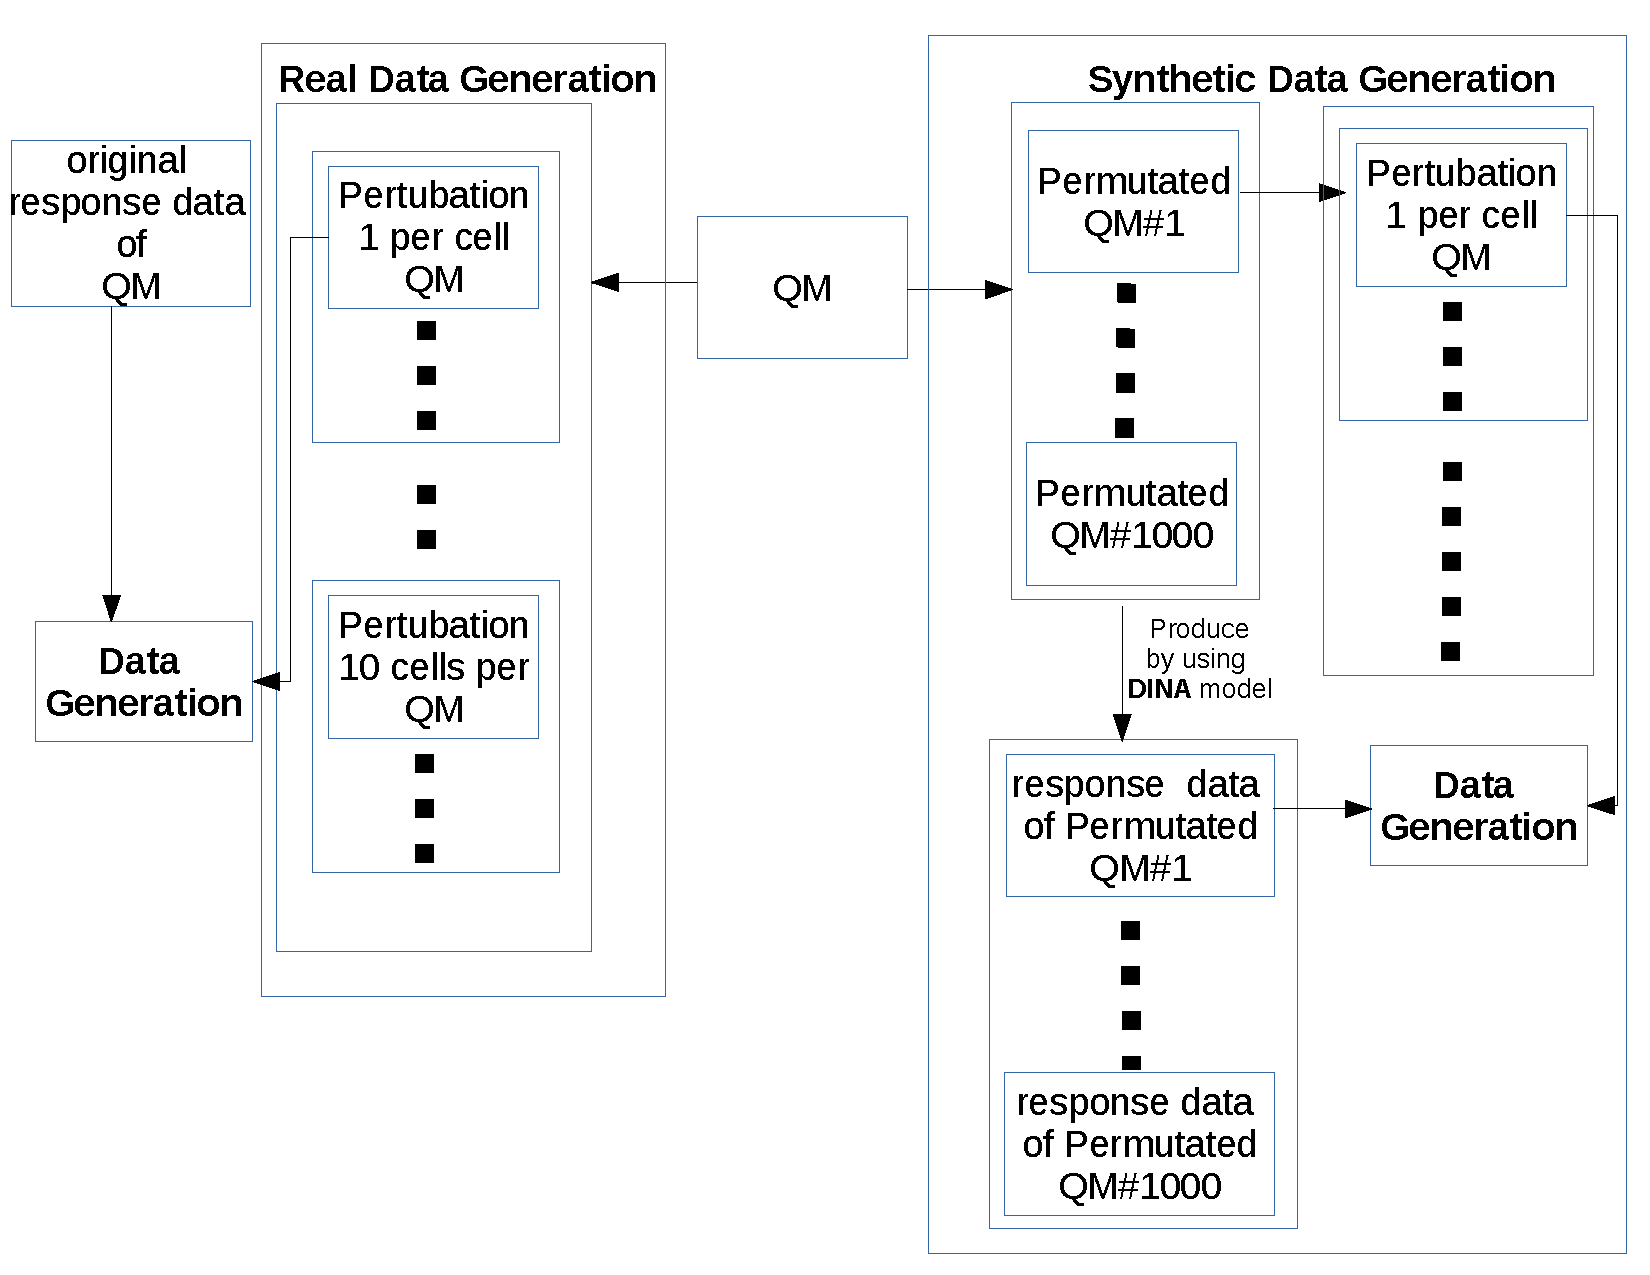
\includegraphics[width=100mm ,scale=0.5]{graph/DG.pdf}
  \caption{Data Generation Procedure of each Q-Matrix~$QM_i$}  \label{fig:DG}
\end{figure}

%%%%%%%%%%%%%%%%%%%%%%%%%%%%%%%%%%%%%%%%%%%%%%%%%%%%%%%%%%%%%%%%%%%%%%%%%%%%%
\subsection{Multi-Label Skills Algorithms}

We transform the proposed outputs and contextual factors from three data driven techniques into a multi-label classification problem. We use synthetic data generated from 1000 permuted matrices for training  and use real data for testing. The procedure for data generation of training and testing is shown in Figure~\ref{fig:DG}. The general idea is to introduce a perturbation in a Q-matrix and to run the refinement algorithms on the perturbed matrix to validate whether the perturbation is identified and whether false perturbations (false alarms) are introduced.  From this process, we can measure the contextual factors of table~\ref{ref:data}, namely the \textit{stickiness} of a cell (tendency of generating a false alarm given a specific refinement algorithm), and which method is most reliable if an item has few or many skills, or if an skill is involved in many items or not.  Given that the Q-matrices to generate the synthetic data are known, this provide the ground truth to do the training.  Noise is introduced to make the data closer to real data and we use the original ratio of 0/1 in the perturbated matrix to create the 1000~permutations.  See~\cite{desmarais2015combining} for details.

Next, we follow the same approach as in~\cite{desmarais2015combining}, but instead of using a decision tree to predict a single cell in a Q-matrix, a multi-label classification algorithm is used for the predicting all skills of an item at once. 

The generality of multi-label problems makes it significantly more complex to solve than traditional single-label (two-class or multi-class) problems. Only a few studies on multi-label learning are reported in the literature, which mainly concern the problems of text categorization, bioinformatics and scene classification. 

Multi-label classification aims to predict a whole vector of labels at once, namely the item skills set in our case. We have a vector of skills for each item in our Q-matrices. So we can transform the proposed outputs of Q-matrices driven from the three refinement techniques and their contextual factors into multi-label classification problem and then we make final prediction by using those features. In this study, we use two multi-label classification methods: binary relevance method (Classifier chain method)~\cite{read2011classifier} by using Naive Bayes classifier, and RAndom k-labELsets(Ensemble method) \cite{Tsoumakas2011random} by using the J48 decision tree algorithm.
 
\subsubsection{Binary Relevance method with Naive Bayes}
The strategy of problem transformation is to use the one-against-all strategy by converting the multi-label problem into several binary classification problems. This approach is known as the binary relevance method (BR)~\cite{read2011classifier}. A method closely related to the BR method is the Classifier Chain method (CC) proposed by Read et al. \cite{read2011classifier}. This method involves~$Q$ binary classifiers linked along a chain. BR transforms any multi-label problem into one binary problem for each label. 

%% \add{\note{moved this paragraph here but needs to be double checked.}\label{notea}}
Let us introduce some notation. Given an instance~$X$ and its associated label set~$l_i \subset |L|$, where its~$l_i$ component of  $ |L|$ takes the value of 1 if~$l_i \in |L|$ and 0 otherwise. In addition, let~$N(x)$ denote the set of~$x$ identified in the training set.

Hence this method trains~$|L|$ binary classifiers~$C_1,...,C_{|L|}$. Each classifier~$C_j$ is responsible for predicting the~$0/1$ association for each corresponding label~$l_j \in L$.\\

BR with Naive Bayes (NB) method makes NB classifiers linked in a chain, such that the classifier for~$l_{i}$ in the chain considers the classes predicted~$l_1,l_2,...,l_{i-1}$ from the previous classifiers as additional attributes. Thus, the feature vector for each binary classifier is extended with the class values (labels) of all previous classifiers in the chain. Each classifier in the chain is trained to learn the association of label~$L_i$
given the features augmented with all previous class labels in the chain, $ C_1;C_1;C_2;...;C_{|L|}$. At classification time, the process starts at~$C_1$, and propagates the predicted classes along   the   chain   such   that   for~$C_i$ it   computes: 
\begin{equation}
P(l_i)= \arg \max_{l_i} P(l_i|X,l_1,l_2,...,l_{i-1}) 
\end{equation}

\subsubsection{RAndom k-labELsets with J48}
The ensemble methods for multi-label learning are developed on top of the common problem transformation or algorithm adaptation methods. The most well known problem transformation ensembles are the RAndom k-labELsets (RAkEL) system by Tsoumakas et al.~\cite{Tsoumakas2011random}. RAkEL constructs each base classifier by considering a small random subset of labels and learning a single-label classifier for the prediction of each element in the power-set of this subset that transformed form multi-label problem. \\

In this experiment we use the single-label J48 classifier, an optimized  implementation of the  C4.5 or improved version of the  C4.5. J48 constructs a Decision tree as an output.  

\section{Error metric}\label{sec:eval-meas-princ}

%% \add{\note{is this notation consistent with the above (note~\ref{notea})?}}
The evaluation of methods for multi-label data requires different metrics than those used in the case of single label data. For the definitions of these metrics, we will consider an evaluation data set of multi-label examples~$(x_i ,Y_i ), i = 1...m, $ where~$ Y_i \subseteq L~$ is the set of true labels and~$ Z_i~$ is the set of predicted labels. This section presents metrics \cite{Tsoumakas2010MLD} that will be used in this experiment for the evaluation of our method. 
%\item Ranking based measurement: are measured based on the ranking scores they received and how far with %respect to the ground truth of multi-label data. It concludes with a subsection on measures that take into %account label hierarchy of the existing label sets. The highest rank is received by the most relevant %label, while the least relevant one, receives the lowest rank.


%% MD: to validate by Sein Minn
%% \subsubsection{Example based metric}
%% %% \add{\note{Single section here}}
%% Example based metrics are calculated over all examples of the evaluation data set, that based on the average differences of the actual and the predicted sets of labels.

\subsubsection{Hamming Loss}: is a measure of how many times an instance label set is misclassified, i.e. a label not belonging to the instance is predicted or a label belonging to the instance is not predicted. The performance is perfect when~$Hamming Loss=0$; the smaller the value of~$Hamming Loss$, the better the performance:
\begin{equation} 
 Hamming Loss= \frac{1}{m}\sum_{i=1}^{m}  \frac{|Z_i\Delta Y_i|}{M}
\end{equation}
where~$\Delta$ stands for the symmetric difference between two label sets. which is the theoretic equivalent of the exclusive disjunction (XOR operation) in Boolean logic for sets.
\subsubsection{Subset Accuracy}
To calculate the accuracy of vector of labels is truly classified. $Subset Accuracy$ is defined as follows:
\begin{equation} 
 Subset Accuracy= \frac{1}{m}\sum_{i=1}^{m}  I(Z_i = Y_i)
\end{equation}
\subsubsection{Example based F-score}: are calculated based on the average differences of the actual and the predicted sets of labels over all examples of the evaluation data set. The performance is perfect when~$Example based F-score = 1$; the bigger the value ,the better the performance:
\begin{equation} 
 Example based F-score= \frac{1}{m}\sum_{i=1}^{m} \frac{2|Y_i \cap Z_i|}{|Z_i|+|Y_i|}
\end{equation}


%\subsection{label based Measurement}
%\subsubsection{One-error}:evaluates how many times the top-ranked label is not in the set of real labels %of the instance.The performance is perfect when~$One Error = 0$; the smaller the value of~$One Error$, the %better the performance:
%\begin{equation} 
% One Error= \frac{1}{m}\sum_{i=1}^{m} \delta (\arg\max_{\lambda \in L} r_i(\lambda))
%\end{equation}
%where
 
 

%$$ \delta (\lambda) = \left\{  \begin{array}{rcl} 1 & \mbox{if} & \lambda \notin Y_i \\ 0 & \mbox{} & %otherwise \end{array}\right.$$


%\subsubsection{Coverage}: measures how far we need on the average to go down the order of labels in order %to cover all the value of labels of the instance. It is loosely related to precision at the level of %perfect recall. The smaller the value 
%of~$Coverage$, the better the performance.
%\begin{equation}
%Coverage = \frac{1}{m}\sum_{i=1}^{m} (\max_{\lambda \in Y_i} r_i(\lambda)-1)
%\end{equation}

%\subsubsection{Ranking Loss}: calculates the average fraction of label pairs that are reversely ranked for %the instance. The performance is perfect when~$Ranking Loss=0$; the smaller the value of~$Ranking %Loss$,the better the performance.
%\begin{equation}
%Ranking Loss = \frac{1}{m}\sum_{i=1}^{m} \frac{1}{|Y_i||\bar{Y_i}|}|\{( \lambda_a , \lambda_b ) : r_i ( %\lambda_a ) > r_i ( \lambda_b ),( \lambda_a , \lambda_b ) \in Y_i \ast Y_i \}|
%\end{equation}
%where~$\bar{Y_i}$ is the complementary set of~$Y_i$ with respect to~$L$.
%\subsubsection{Average Precision}: evaluates the average fraction of labels ranked above a particular %label~$y \in Y$ which actually are in~$Y$. Information Retrieval (IR) systems use it to evaluate the %document ranking performance for query retrieval [10]. The performance is perfect when~$ Average Precision %= 1$; the bigger the value ,the better the performance.
%\begin{equation}
%Average Precision = \frac{1}{m}\sum_{i=1}^{m} \frac{1}{|Y_i|}| \sum_{\lambda \in Y_i} \frac{|\{ %\acute{\lambda} \in Y_i : r_i (\acute{\lambda})\leq r_i ( \lambda )  \}|}{r_i(\lambda)}
%\end{equation}

\section{Experimental Study}\label{sec:experimental-study}

For the sake of comparison, we use the same datasets as the ones used in Desmarais et al.\ (2015)~\cite{tatsuoka1983rule,desmarais2015combining}. It is a well known data set in
fraction algebra from Tatsuoka's work (Tatsuoka, 1984)\cite{tatsuoka1983rule}. It consists 3 expert-driven Q-matrices and one SVD driven Q-matrix with a same data set.These allow us to analyze possibility of different models (Q-matrices) over the same data source.Table~\ref{tab:qm} provides the basic information and source of each dataset.   

\begin{table} 
\begin{center}
  \caption{Q-matrix for validation \& explanation of category}\label{tab:qm}
  \begin{tabular}{|ccccp{4cm}<{\raggedright}|}
  \hline
  \toprule
\multirow{2}{*}{Q-Matrices} & \multicolumn{3}{c}{Number of} & \multirow{2}{*|}{Description} \\
  \cline{2-4}
  & Skills &  Items & \multicolumn{1}{c}{Cases} & \\
  \midrule
QM1 & 3 & 11 & 536 & {Expert driven from \cite{henson2009defining} } \\
	\hline
QM2 & 5 & 11 & 536 & {Expert driven from \cite{de2008empirically} } \\  
 	\hline
QM3 & 3 & 11 & 536 & {Expert driven from \cite{CDM}} \\  
  	\hline 
QM4 & 3 & 11 & 536 & {Data driven, SVD based} \\  
  	\hline
  	\end{tabular}  
\end{center}	
\end{table}

\begin{figure}\label{fig:RP}
  \centering
    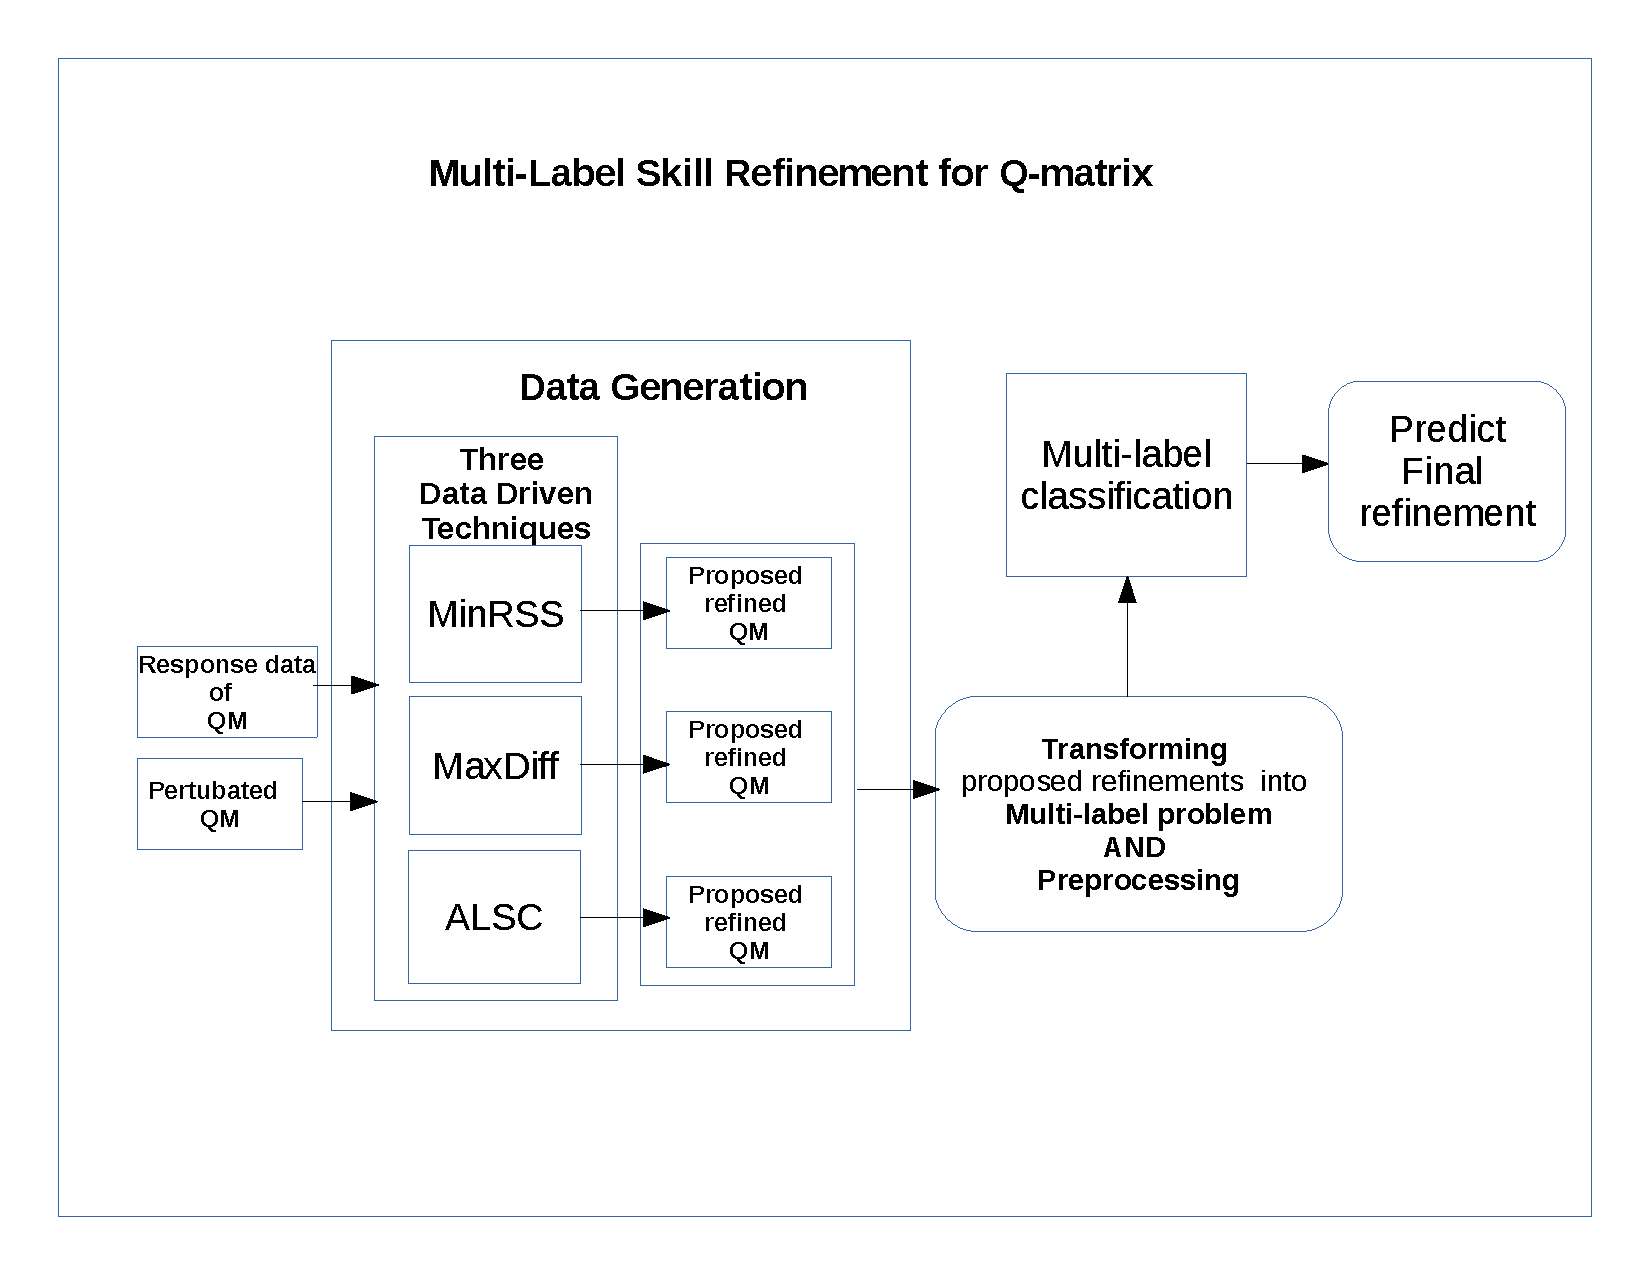
\includegraphics[width=100 mm ,scale=0.25]{graph/RP.pdf}
  \caption{Refinement Procedure of each Q-Matrix~$QM_i$ }
\end{figure}



\begin {table}[h]
\scriptsize
\centering
\begin{tabular}{c|c|c|c|c|c}	
	\hline\hline	
QM & MinRSS & MaxDiff & ALSC & RAkEL & BR   \\ \hline
qm1 & 0.01 & 0.02 & 0.01 & 0.00 & 0.00 \\
qm2 & 0.02 & 0.04 & 0.06 & 0.01 & 0.01  \\
qm3 & 0.00 & 0.02 & 0.01 & 0.00 & 0.00   \\
qm4 & 0.01 & 0.02 & 0.01 & 0.00 & 0.01  \\  \hline\hline
\end{tabular}
\caption {Hamming Loss result of Synthetic data (single perturbation)} \label{ref:Syn_HL} 
\end{table}




\begin {table}[h]
\scriptsize
\centering
\begin{tabular}{c|c|c|c|c|c}	
	\hline\hline	
QM  & MinRSS  & MaxDiff  & ALSC  & RAkEL & BR    \\  \hline
qm1  & 0.98 & 0.95 & 0.97 & 0.99 & 0.99  \\
qm2  & 0.90 & 0.83 & 0.72 & 0.97 & 0.94  \\
qm3  & 0.99 & 0.96 & 0.99 & 1.00 & 1.00  \\
qm4  & 0.98 &  0.94 & 0.98 & 0.99 & 0.98  \\
\hline\hline
\end{tabular}
\caption {SubSet Accuracy result of Synthetic data (single perturbation)} \label{ref:Syn_SA} 
\end{table}



\begin {table}[h]
\scriptsize
\centering
\begin{tabular}{c|c|c|c|c|c}	
	\hline\hline	
 QM  &  MinRSS & MaxDiff  &  ALSC  &  RAkEL &  BR  \\ 
 qm1  & 0.99 & 0.98 & 0.99 & 1.00 & 1.00  \\  
 qm2  & 0.98 & 0.98 & 0.96 & 1.00 & 0.99  \\
 qm3  & 1.00 & 0.98 & 0.99 & 1.00 & 1.00  \\
 qm4  & 0.99 & 0.98 & 0.99 & 1.00 & 0.99  \\
\hline\hline
\end{tabular}
\caption {Macro averaged F-measure result of Synthetic data (single perturbation)} \label{ref:Syn_FM} 
\end{table}

All experiments were done with 10 fold cross validation. 
We relied on the CDM \cite{CDM} and NPCD packages which provided both the code for three basic data driven techniques and the data, and mulan \cite{Tsoumakas2010MLD} for multi-label classification.

  We use Hamming loss, Subset Accuracy and Example based F-measure to assess the performance of the different algorithms.\\


 The experimental results are reported in Tables [\ref{ref:Syn_HL},\ref{ref:Syn_SA},\ref{ref:Syn_FM}] for synthetic data, and in  Figures [\ref{fig:HLforReal},\ref{fig:SAforReal},\ref{fig:FMforReal}] for real data. Four variations of the two multi-label approaches are reported for both real and synthetic data (BR.$n$ and RAkEL.$n$).  They correspond to different training data.  The four variations respectively contain:

\begin{itemize}   
	\item[BR.1/RAkEL.1]: item number, outputs from three different basic algorithms
	\item[BR.2/RAkEL.2]: item number, stickiness factors from three different algorithms	  
	\item[BR.3/RAkEL.3]: combination of item number, outputs, row sum and column sums.	  
	\item[BR.4/RAkEL.4]: combination of item number, outputs,stickiness factors, row sum and column sums.	  
\end{itemize}

For synthetic data, a single cell is perturbed. We can see from Tables~[\ref{ref:Syn_HL},\ref{ref:Syn_SA},\ref{ref:Syn_FM}] that most of multi-label skill refinement methods can recover over 99\% for all Q-matrices and even the performance reaches 100\% in terms of subset accuracy and macro averaged F-measure.  The standard deviations of all values except the ones marked with stars are below 0.05 (*$\rightarrow sd<0.01$, **$\rightarrow sd<0.02$, ***$\rightarrow sd<0.05$), which makes the vast majority of differences statistically significant. Clearly, all methods using multi-label refinement algorithms perform much better than any single method and the results are also substantially better than those of the single-cell decision tree method reported in~\cite{desmarais2015combining}.

For real data, multiple perturbations are introduced and the results are shown as figures to better visualize the trends as a function of the number of perturbations.   A logit scale is used which can be considered a good estimate of the relative remaining error on a scale of~$[0,1]$ (for eg., it displays a relative error reduction in accuracy from~0.90 to~0.95 as similar to the reduction from~0.99 to~0.995). The black lines show the results of the three individual refinement algorithms, and the coloured lines show the multi-label algorithms results.  

As expected, the performance declines with the number of perturbations. BR.1 and BR.2 show the best performances in general.  However, the results for QM1 shows that the MaxDiff method has a performance relatively close to the these two methods, BR.1 and BR.1

These results reveal a trend in the performance of our method: it underperforms with fewer skills. For eg., the 5-skills QM2 shows a better performance than the 3-skills QM1, QM3 and QM4. Furthermore, QM1 has only two skills that really vary across items (skill~1 is required by all) and it is the method for which the performance of the multi-label approach is the worst.

\begin{figure}
  \centering
    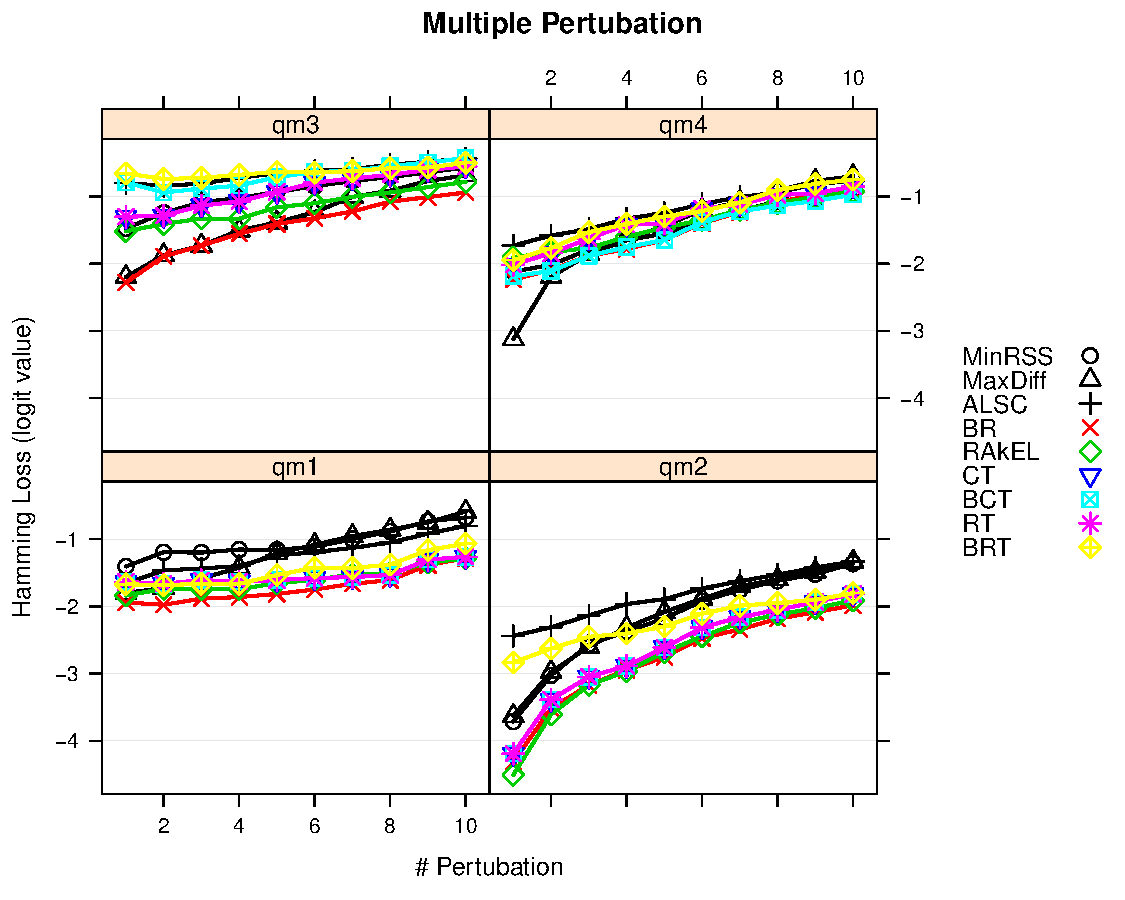
\includegraphics[width=100 mm ,scale=0.25]{graph/HL.pdf}
  \caption{Real data: Logit value of Hamming loss as a function of the number of perturbations}\label{fig:HLforReal}
\end{figure}

\begin{figure}
  \centering
    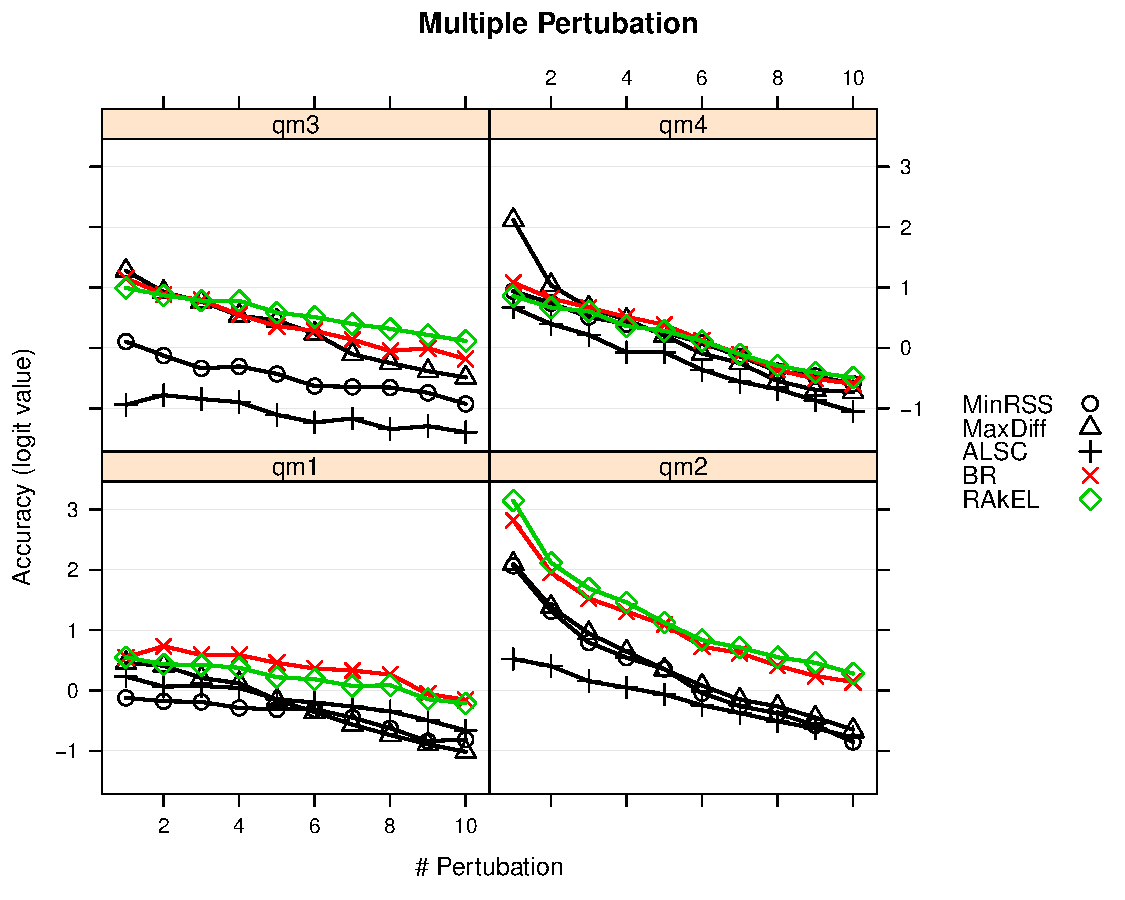
\includegraphics[width=100 mm ,scale=0.25]{graph/SA.pdf}
  \caption{Real data: Logit value of Subset Accuracy as a function of the number of perturbations}\label{fig:SAforReal}
\end{figure}

\begin{figure}
  \centering
    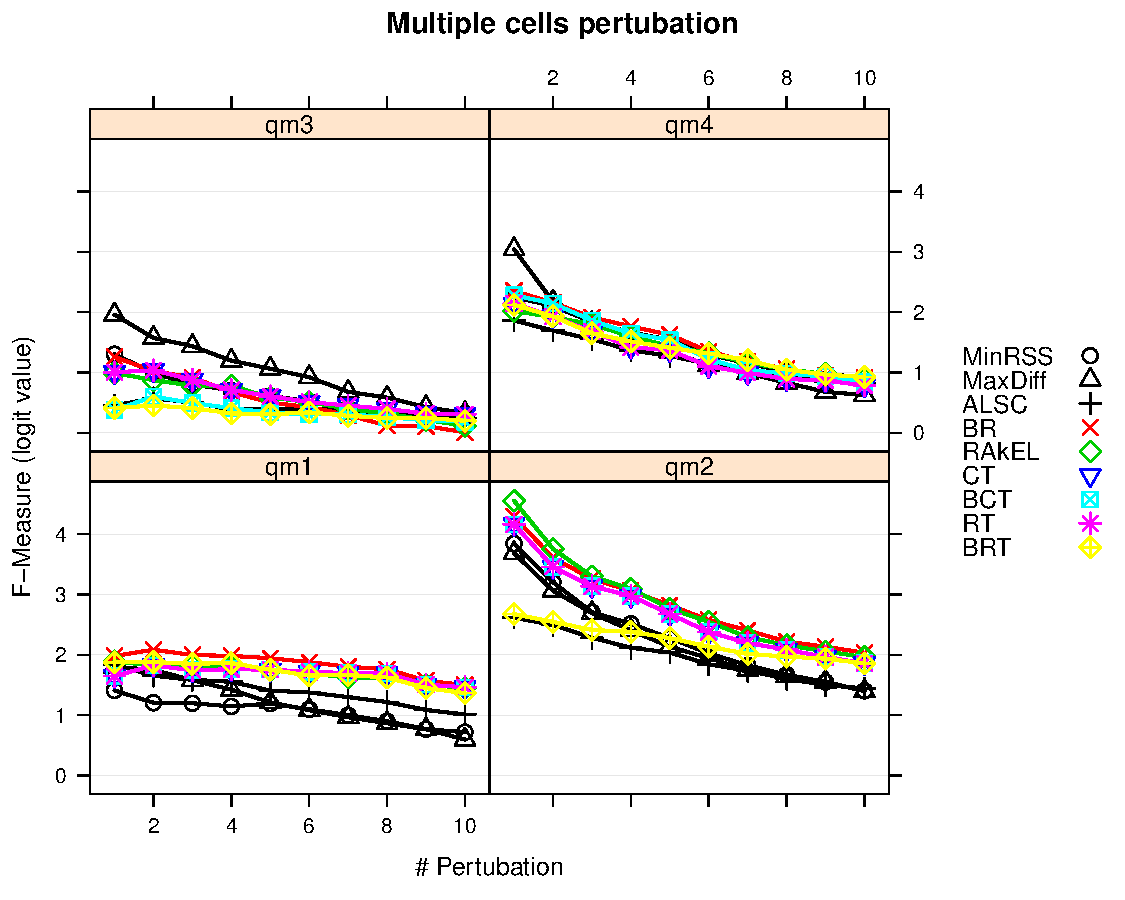
\includegraphics[width=100 mm ,scale=0.25]{graph/FM.pdf}
    \caption{Real data: Logit value of Example-based F-measure as a function of the number of perturbations}\label{fig:FMforReal}
\end{figure}



%\begin{subfigures}\label{fig:Measurement2}
%\begin{figure}[H]  
%  \centering
%    \includegraphics[width=\textwidth ,scale=0.4]{graph/OE.pdf}
%  \caption{Logit value of One Error}
%\end{figure}

%\begin{figure}[H]  
%  \centering
%    \includegraphics[width=\textwidth ,scale=0.4]{graph/Cover.pdf}
%  \caption{Coverage}
%\end{figure}

%\begin{figure}[H]  
%  \centering
%    \includegraphics[width=\textwidth ,scale=0.4]{graph/RL.pdf}
%    \caption{Logit value of Ranking Loss}
%\end{figure}
%\begin{figure}[H]    
%  \centering
%    \includegraphics[width=\textwidth ,scale=0.4]{graph/AP.pdf}
%    \caption{Logit value of Average Precision}
%\end{figure}
%\end{subfigures}

\section{Conclusion and Future Work}\label{sec:conclusion--future}
In this paper, we represent the multi-label skills to tasks refinement methods, that combine three data driven techniques and two multi-label classification techniques. Experiments with 3 expert driven Q-matrices and 1 Q-matrix driven from SVD, show the proposed refinement methods generally outperform the stand alone refinement algorithms. However, for real data, a Q-matrix with only two discriminant skills does not prove more effective than the MaxDiff refinement algorithm and the general pattern suggests the more skills involved, the better the BR.1 and BR.2 approaches perform.

As with previous work with ensemble techniques \cite{desmarais2015combining,pengxu2016}, the experiments were conducted with static data, where the student does not learn during the data gathering process.  Dealing with dynamic data, which is typical of traces collected from learning environments, imposes another challenge and a few researchers have done valuable work in that direction \cite{matsudamachine2015,gonzalez2015modeling,aleven2013knowledge}.

%%%%%%%%%%%%%%%%%%%%%%%%%%%%%%%%%%%%%%%%%%%%%%%%%%%%%%%%%%%%%%%%%%%%%%%%%%%%%
\section{Acknowledgements}

This work is funded by the NSERC Discovery funding awarded to the second author.

%%%%%%%%%%%%%%%%%%%%%%%%%%%%%%%%%%%%%%%%%%%%%%%%%%%%%%%%%%%%%%%%%%%%%%%%%%%%%%%
\bibliographystyle{splncs}
\bibliography{biblio}

%%%%%%%%%%%%%%%%%%%%%%%%%%%%%%%%%%%%%%%%%%%%%%%%%%%%%%%%%%%%%%%%%%%%%%%%%%%%%%%
All links were last followed on June 20, 2016.
\end{document}
